% Source-derived chapter 02: Geometry of the spectral side
% Original source: tates-thesis-de-rham-setting
\chapter{Geometry of the spectral side}
\label{tates-thesis-de-rham-setting-chapter-02}
\source{tates-thesis-de-rham-setting}

\begin{remark}[Source section]
\label{tates-thesis-de-rham-setting-chapter-02-source}
\source{tates-thesis-de-rham-setting}
\source{tates-thesis-de-rham-setting}
This chapter reproduces the corresponding section of the retrieved
LaTeX source, including its definitions, statements, examples, and
proofs. It has not yet been translated into Lean.
\notready
\end{remark}

% The source section title was: Geometry of the spectral side
\label{s:spectral}
\source{tates-thesis-de-rham-setting}

\subsection{Overview}

In this section, we define $\sY$ and establish our main algebro-geometric tools
for studying its coherent sheaves.

Here is a more detailed overview of this section. 

In \S \ref{ss:jet-notation}, we give background on jet and loop spaces,
essentially setting up notation for later use.
In \S \ref{ss:rk1-ls}, we give background on $\LocSys_{\bG_m}$.
In \S \ref{ss:y-defin}, we define $\sY$. In \S \ref{ss:y-trun},
we introduce variants of $\sY$ that are more traditional objects
of algebraic geometry. In \S \ref{ss:flatness}, we prove a series 
of flatness results; these are the key tools for studying $\sY$ and
its coherent sheaves. 

The remainder of the section consists of a series of codas, essentially 
developing material and notation for later reference. These may be skipped
at first pass and referred to as needed. In \S \ref{ss:y-not}, we introduce
additional notation for later reference. In \S \ref{ss:fund}, we deduce
some exact sequences from our flatness results; these will be used
later in some inductive arguments. In \S \ref{ss:un}, we describe
certain well-behaved opens in $\sZ^{\leq n}$. 
In \S \ref{ss:coords}, we explicitly describe $\sY$ using
generators and relations. Finally, in \S \ref{ss:rs-sketch}, we draw pictures
explicitly describing the geometry in the regular singular situation.

\subsection{Notation for jet and loop spaces}\label{ss:jet-notation}
\source{tates-thesis-de-rham-setting}

\subsubsection{}

For a commutative DG algebra $A \in \ComAlg$, 
$A[[t]] \in \ComAlg$ is defined as 
$(\lim_n A \otimes k[[t]]/t^n)$ and $A((t))$ is defined
as $A[[t]] \otimes_{k[[t]]} k((t))$. We also let
$A[[t]]/t^n \coloneqq A \otimes_k k[[t]]/t^n$.
% emph: notation is derived?

\subsubsection{}

For a prestack $Z$, 
$\fL Z \in \PreStk \coloneqq \TwoHom(\AffSch^{op},\Gpd)$ denote the functor:
%
\[
\Spec(A) \mapsto \Hom_{\AffSch}(\Spec(A((t))),Z).
\]

\noindent Similarly, we let $\fL^+ Z$ denote the functor:
%
\[
\Spec(A) \mapsto \Hom_{\AffSch}(\Spec(A[[t]]),Z).
\]

For $n \geq 0$, we let $\fL_n^+$ denote the functor:
%
\[
\Spec(A) \mapsto \Hom_{\AffSch}(\Spec(A[[t]]/t^n),Z).
\]

There is an evident comparison map:
%
\[
\vareps_Z:\fL^+ Z \to \underset{n}{\lim} \, \fL_n^+ Z.
\]

We often use the following lemma without mention.

\begin{lem}
\source{tates-thesis-de-rham-setting}
\notready

For $Z$ an algebraic stack of 
the form $Y/G$ with $Y$ affine and $G$ an affine 
algebraic group, the map $\kappa_Z$ is an isomorphism.

\end{lem}

\begin{proof}

The result is obvious when $Z = Y$ is affine.
For $Z = \bB G$, we refer e.g. to \cite{cpsii} Lemma 2.12.1.
The argument from \emph{loc. cit}. immediately
extends to the general form of $Y$ considered here.

\end{proof}

\begin{rem}
\source{tates-thesis-de-rham-setting}
\notready

In fact, this result is true much more 
generally for Noetherian algebraic
stacks with affine diagonals: see \cite{bhatt-hl} Corollary 1.5.

\end{rem}

\begin{notation}
\source{tates-thesis-de-rham-setting}
\notready

We often let $\ev:\fL^+ Z \to \fL_1^+ Z = Z$ 
denote the evaluation map.

\end{notation}

\subsubsection{}

We have the following basic representability result.

\begin{prop}
\source{tates-thesis-de-rham-setting}
\notready\label{p:loop-rep}
\source{tates-thesis-de-rham-setting}

Suppose $Z$ is an affine scheme almost of finite type.
Then $\fL^+ Z$ is an affine scheme and $\fL Z$ is an 
indscheme.

\end{prop}

\subsubsection{}

We have the following variant of the above.

Suppose $Z$ is equipped with a $\bG_m$-action. 
We let $\fL Zdt \in \PreStk$ denote the functor:
%
\[
\fL Z dt \coloneqq \fL(Z/\bG_m) \underset{\fL \bB \bG_m}{\times} \Spec(k)
\]

\noindent where $\Spec(k) \to \fL \bB \bG_m$ corresponds to the
(continuous) tangent sheaf $T_{\o{\sD}}$ on $\o{\sD}$.
We define $\fL^+Z dt$ similarly. A choice of trivialization
of $T_{\o{\sD}}$ defines an isomorphism $\fL Z dt \simeq \fL Z$
identifying $\fL^+ Z dt$ and $\fL^+ Z$; in particular,
Proposition \ref{p:loop-rep} applies in this setting.

Informally, $\fL Z dt$ parametrizes sections of
the fiber bundle $\o{\Theta}(\Omega_{\o{\sD}}^1) \overset{\bG_m}{\times} Z \to 
\o{\sD}$, where $\Omega_{\o{\sD}}^1$ is the line bundle 
of (continuous) 1-forms on $\o{\sD}$ and $\Theta(-)$ 
(resp. $\o{\Theta}$) denotes the
(resp. punctured) total space of a line bundle. 

\begin{example}
\source{tates-thesis-de-rham-setting}
\notready

$\fL \bA^1$ is the algebro-geometric version of the space of Laurent
series, while $\fL \bA^1 dt$ is the algebro-geometric verison of the
space of 1-forms on the punctured disc (for the standard $\bG_m$-action 
on $\bA^1$ by homotheties). Similarly, $\fL \bG_m$ is the algebro-geometric
version of the space of invertible Laurent series.
One easily finds that these indschemes are formally smooth and classical.

\end{example}

\subsection{Rank $1$ local systems}\label{ss:rk1-ls}
\source{tates-thesis-de-rham-setting}

We now give a detailed study of $\LocSys_{\bG_m}$, the moduli space of 
rank $1$ local systems on the punctured disc. This material is well-known,
but it is convenient to review to introduce notation and constructions
we will need in the more complicated setting of our space $\sY$.

\subsubsection{}

We define $\LocSys_{\bG_m}$ as follows.

We have a map $\fL \bG_m \to \fL \bA^1 dt$ sending
$f \in \fL \bG_m$ to $d\log(f)$, cf. \cite{locsys} \S 1.12.
This map is a map of (classical) group indschemes, where
$\fL \bA^1 dt$ is given its natural additive structure.

We define $\LocSys_{\bG_m}$ as the stack\footnote{I.e., we sheafify
for the fppf topology. It is equivalent to sheafify for the 
Zariski topology as $\Ker(\fL^+ \bG_m \to \bG_m)$ is pro-unipotent.
For the same reason, the resulting prestack is a sheaf for the 
fpqc topology. In other words, there is no room for ambiguity in 
sheafifying.}
quotient $\fL \bA^1 dt/\fL \bG_m$. 

\begin{rem}
\source{tates-thesis-de-rham-setting}
\notready

For normalization purposes, we remark that for 
a point $\omega \in \fL \bA^1 dt$, we consider 
$\nabla = d - \omega$ as the corresponding rank $1$ connection
(on the trivial line bundle).

\end{rem}

\subsubsection{}

We need variants of $\LocSys_{\bG_m}$ as well.

Define:
%
\[
\LocSys_{\bG_m,\log} \coloneqq 
\LocSys_{\bG_m} \underset{\fL \bB\bG_m}{\times} \fL^+ \bB \bG_m = 
\fL \bA^1 dt/\fL^+ \bG_m.
\]

\noindent This is the moduli space of line bundles on the
disc with a connection on the punctured disc. 

There is an
evident action of $\Gr_{\bG_m} \coloneqq \fL \bG_m/\fL^+ \bG_m$ 
on $\LocSys_{\bG_m,\log}$ such that 
$\LocSys_{\bG_m} = \LocSys_{\bG_m,\log}/\Gr_{\bG_m}$.

\subsubsection{}

Define $\fL^{pol} \bA^1 dt$ as the quotient
$\fL \bA^1 dt / \fL^+\bA^1 dt$, the quotient being with respect
to the additive structure. In other words, $\fL^{pol} \bA^1 dt$
parametrizes polar parts of differential forms on the disc.
Note that $\fL^{pol} \bA^1 dt$ is an indscheme of ind-finite type.

As $d\log$ maps $\fL^+ \bG_m$ into $\fL^+ \bA^1 dt$, the
projection map:
%
\[
\fL \bA^1 dt \to \fL^{pol} \bA^1 dt
\]

\noindent intertwines the gauge action of $\fL^+ \bG_m$ on 
the left hand side with its trivial action on the right hand
side. Therefore, we obtain a canonical map:
%
\[
\Pol: \LocSys_{\bG_m,\log} \to \fL^{pol} \bA^1 dt.
\]

\noindent This map takes the polar part of a connection.

\subsubsection{}

By construction, there is a map:
%
\[
\LocSys_{\bG_m,\log} \to \bB \fL^+ \bG_m \xar{\ev} \bB \bG_m.
\]

\noindent This map sends a pair $(\sL,\nabla)$ (with $\sL$ a line
bundle on the disc and $\nabla$ its connection on the punctured
disc) to the fiber of $\sL$ at the origin.

The following result is well-known.

\begin{prop}
\source{tates-thesis-de-rham-setting}
\notready\label{p:locsys-log}
\source{tates-thesis-de-rham-setting}

The map:
%
\[
\LocSys_{\bG_m,\log} \to \fL^{pol} \bA^1 dt \times \bB \bG_m
\]

\noindent is an isomorphism.

\end{prop}

\begin{proof}

The map $\fL^+ \bG_m \xar{d\log,\ev} \fL^+ \bA^1 dt \times \bG_m$
is easily seen to be an isomorphism. The result is immediate
from here.

\end{proof}

\subsubsection{}

We now deduce a similar description of $\LocSys_{\bG_m}$
from Proposition \ref{p:locsys-log}.

There is a canonical residue map 
$\Res:\fL^{pol} \bA^1 dt \to \bA^1$. There is a canonical projection
$\fL^{pol} \bA^1 dt \to \Ker(\Res)$ as the latter identifies
with $\fL \bA^1 dt/t^{-1} \cdot \fL^+ \bA^1 dt$,
so we obtain a product decomposition:
%
\[
\fL^{pol} \bA^1 dt = \bA^1 \times \Ker(\Res).
\]

\begin{prop}
\source{tates-thesis-de-rham-setting}
\notready\label{p:locsys}
\source{tates-thesis-de-rham-setting}

There is an isomorphism $\LocSys_{\bG_m} \simeq 
\bA^1/\bZ \times \Ker(\Res)_{dR} \times \bB \bG_m$ fitting
into a commutative diagram:
%
\[
\xymatrix{
\LocSys_{\bG_m,\log} \ar[rr]^{\text{Prop. \ref{p:locsys-log}}} 
\ar[d] & & \fL^{pol} \bA^1 dt \times \bB \bG_m \ar[d] \\
\LocSys_{\bG_m} \ar[rr]^{\simeq}
& &
\bA^1/\bZ \times \Ker(\Res)_{dR} \times \bB \bG_m
}
\]

\end{prop}

\begin{proof}

There is a canonical homomorphism
$\Gr_{\bG_m} \to \bZ$ given by minus\footnote{This sign is included to match
with standard normalizations.} the valuation map. This map splits 
canonically as well: $\bZ = \Gr_{\bG_m}^{red}$.
Therefore, we obtain a canonical product decomposition:
%
\[
\Gr_{\bG_m}^{red} = \bZ \times \Gr_{\bG_m}^{\circ}
\]

\noindent for $\Gr_{\bG_m}^{\circ}$ the connected component
of the identity. Here we consider $\bZ$ as a discrete indscheme
over $k$ in the natural way, i.e., as $\coprod_{n \in \bZ} \Spec(k)$.

We have a commutative diagram:
%
\[
\xymatrix{
\Gr_{\bG_m} \ar[r]^{d\log} \ar@{=}[d] & 
\fL^{pol} \bA^1 dt \ar@{=}[d] \\
\bZ \times \Gr_{\bG_m}^{\circ} \ar[r] 
& \bA^1 \times \Ker(\Res) 
}
\]

\noindent where the bottom map is obtained as the product
of the homomorphisms $\bZ \into \bA^1$ and 
$d\log:\Gr_{\bG_m}^{\circ} \to \Ker(\Res)$. The latter
is easily seen to induce an isomorphism between
$\Gr_{\bG_m}^{\circ}$ and the formal group 
$\Ker(\Res)_0^{\wedge}$ of $\Ker(\Res)$. This gives the claim.

\end{proof}

\begin{rem}
\source{tates-thesis-de-rham-setting}
\notready

This isomorphism actually depends mildly on the choice of uniformizer $t$;
this is needed to trivialize the action of 
$\Gr_{\bG_m}$ on the $\bB \bG_m$-factor. 

\end{rem}

\subsubsection{}

We will also use \emph{truncated} versions of the above spaces in 
which we bound the irregularity of our local systems.

We fix $n \in \bZ^{\geq 0}$ in what follows.

\subsubsection{}

Define $\fL^{\leq n} \bA^1 dt \subset \fL \bA^1 dt$ as the
classical closed subscheme whose points are differential 
forms with poles of order at most $n$. Therefore, 
$\fL^{\leq n} \bA^1 dt$ is the image of $\fL^+ \bA^1 dt$ under the
map $t^{-n} \cdot -:\fL \bA^1 dt \to \fL \bA^1 dt$.

We similarly define $\fL^{pol,\leq n} \bA^1 dt$ as 
$\fL^{\leq n} \bA^1 dt/\fL^+ \bA^1 dt$. For $n > 0$, we define
$\Ker(\Res)^{\leq n}$ as $\Ker(\fL^{\leq n} \bA^1 dt \to \bA^1)$.

\subsubsection{}\label{ss:loop-gr-trun}
\source{tates-thesis-de-rham-setting}

For $n>0$, define $\fL^{\leq n} \bG_m$ as the fiber product:
%
\[
\fL^{\leq n} \bG_m \underset{\fL \bA^1 dt}{\times} \fL^{\leq n} \bA^1 dt
\]

\noindent where we are using $d\log:\fL \bG_m \to \fL \bA^1 dt$.

For\footnote{We separate the cases to be derivedly correct.} 
$n = 0$, define $\fL^{\leq 0} \bG_m$ as $\fL^+ \bG_m$.

Finally, define $\Gr_{\bG_m}^{\leq n}$ as $\fL^{\leq n}\bG_m/\fL^+\bG_m$.

\begin{lem}
\source{tates-thesis-de-rham-setting}
\notready

$\fL^{\leq n} \bG_m$ is a formally smooth classical indscheme.

\end{lem}

\begin{proof}

It suffices to show the same for $\Gr_{\bG_m}^{\leq n}$.

As in the proof of Proposition \ref{p:locsys}, the map
$\Gr_{\bG_m} \xar{d\log} \fL \bA^1 dt \to \Ker(\Res)$ induces an
isomorphism:
%
\[
\Gr_{\bG_m}^{\leq n} \isom \bZ \times (\Ker(\Res)^{\leq n})_0^{\wedge}.
\]

\noindent Here $\Ker(\Res)^{\leq n}$
is defined as the kernel of the
residue on polar forms with poles of order $\leq n$. 
As the latter is an affine space, its formal completion at the origin
is formally smooth and classical. This gives the claim.

\end{proof}

\subsubsection{}

Next, define $\LocSys_{\bG_m}^{\leq n}$ as the quotient
$\fL^{\leq n} \bA^1 dt/\fL^{\leq n} \bG_m$ under the gauge action.
We similarly define $\LocSys_{\bG_m,\log}^{\leq n}$ as 
$\fL^{\leq n} \bA^1 dt/\fL^+ \bG_m$. By definition, 
we have a Cartesian diagram:

\begin{prop}
\source{tates-thesis-de-rham-setting}
\notready\label{p:locsys-trun}
\source{tates-thesis-de-rham-setting}

The isomorphisms from Propositions \ref{p:locsys-log} and \ref{p:locsys}
induce further isomorphisms:
%
\[
\xymatrix{
\LocSys_{\bG_m,\log}^{\leq n} \ar[rr]^{\simeq}
\ar[d] & & \fL^{pol,\leq n} \bA^1 dt \times \bB \bG_m \ar[d] \\
\LocSys_{\bG_m,\log} \ar[rr]^{\simeq}
 & & \fL^{pol} \bA^1 dt \times \bB \bG_m
}
\]

\noindent and:
%
\[
\xymatrix{
\LocSys_{\bG_m}^{\leq n} \ar[rr]^{\simeq} \ar[d] 
& &
\bA^1/\bZ \times \Ker(\Res)_{dR}^{\leq n} \times \bB \bG_m \ar[d] \\
\LocSys_{\bG_m} \ar[rr]^{\simeq}
& &
\bA^1/\bZ \times \Ker(\Res)_{dR} \times \bB \bG_m.
}
\]

\end{prop}

This result is clear from our earlier analysis.


\subsection{Definition of $\sY$}\label{ss:y-defin}
\source{tates-thesis-de-rham-setting}

\subsubsection{}

We define $\sY$, the moduli of rank $1$ de Rham local systems on $\o{\sD}$
with a flat section, as follows.

First, observe that we have a map $d:\fL \bA^1 \to \fL \bA^1 dt$
defined by the exterior derivative on $\o{\sD}$.
We also have a product map $\fL \bA^1 \times \fL \bA^1 dt \to \fL \bA^1 dt$
coming from the product $\bA^1 \times \bA^1 \to \bA^1$.

Let $\sY^{\prime}$ denote the equalizer:
%
\[
\sY^{\prime} \coloneqq \on{Eq}
\big(\fL \bA^1 \times \fL \bA^1 dt 
\underset{(g,\omega) \mapsto g\omega}{\overset{d\circ \pi_1}{\rightrightarrows}}
\fL \bA^1 dt\big) \in \PreStk
\]

\noindent We emphasize that this is a \emph{derived} equalizer;
although the terms appearing are classical indschemes, this
equalizer is a priori a DG indscheme.

There is a canonical $\fL \bG_m$-action on $\sY^{\prime}$,
heuristically given by the formula:
%
\[
(f \in \fL \bG_m,(g,\omega) \in \sY^{\prime}) \mapsto 
(fg,\omega+d\log(f)).
\]

\noindent We will define this action more rigorously below,
but in the meantime, we define:
%
\[
\sY \coloneqq \sY^{\prime}/\fL \bG_m.
\]

\begin{rem}
\source{tates-thesis-de-rham-setting}
\notready

Let us explain the above formulae.

Note that $\sY^{\prime}$ by definition parametrizes pairs
$(g \in \fL\bA^1, \omega \in \fL \bA^1 dt) $ with
$dg = g\omega$, which we can rewrite as 
$\nabla g = 0$ for $\nabla \coloneqq d - \omega$. 
This data amounts to a connection on the trivial bundle on $\o{\sD}$ 
(corresponding to $\omega$) and a flat section (corresponding to $g$). 

Quotienting by $\fL \bG_m$ amounts to modding out by gauge transformation,
i.e., not fixing a trivialization on our line bundle on $\o{\sD}$.

\end{rem}

\subsubsection{}\label{ss:action-rigorous}
\source{tates-thesis-de-rham-setting}

Above, we did not define the action of $\fL \bG_m$ on $\sY^{\prime}$
completely rigorously: as $\sY^{\prime}$ is a priori DG, such
formulae are not sufficient. (In fact, using Theorem \ref{t:cl}, $\sY^{\prime}$
is classical, and the implicit anxiety here is not needed.)

Here are two approaches. 

First, in \cite{dennis-punctured-disc}, 
Gaitsgory defines a prestack $\Maps(\o{\sD}_{dR},Y)$ for any 
prestack $Y$. Taking $Y = \bA^1/\bG_m$ then immediately gives the definition
of $\sY$ as $\Maps(\o{\sD}_{dR},\bA^1/\bG_m)$. (One readily
finds $\Maps(\o{\sD}_{dR},\bB \bG_m) = \LocSys_{\bG_m}$ and
$\sY^{\prime} = \Maps(\o{\sD}_{dR},\bA^1/\bG_m) 
\times_{\Maps(\o{\sD}_{dR},\bB \bG_m)} \Omega_{\bG_m}^1$, consistent
with our constructions.)

We prefer an alternative approach that we find more explicit, and that we
describe in full detail here. The reader who is not concerned about
homotopical details (which are not serious anyway by Theorem \ref{t:cl})
may skip this material.

Below, we make various constructions with $\fL \bA^1 \times \fL \bA^1 dt$. Here we may
just work with formulae as this indscheme is classical.

We consider two monoid structures on $\fL \bA^1 \times \fL \bA^1 dt$. 
The first has product:
%
\[
(g,\omega) \dot (\tilde{g},\tilde{\omega}) \coloneqq 
(g\tilde{g},\omega+\tilde{\omega})
\]

\noindent while the second has product:
%
\[
(g,\omega) \star (\tilde{g},\tilde{\omega}) \coloneqq 
(g\tilde{g},g\tilde{\omega}+\tilde{g}\omega).
\]

\noindent Moreover, the map:
%
\[
\begin{gathered}
\mu:\fL \bA^1 \times \fL \bA^1 dt \to \fL \bA^1 \times \fL \bA^1 dt \\
(g,\omega) \mapsto (g,dg-g\omega)
\end{gathered}
\]

\noindent is a map of monoids $(\fL \bA^1 \times \fL \bA^1 dt,\dot) \to 
(\fL \bA^1 \times \fL \bA^1 dt,\star)$.

We obtain a commutative diagram of maps of monoids:
%
\[
\xymatrix{
\fL \bG_m \ar[rrr]^(.4){f \mapsto (f,d\log(f))} 
\ar[d] &&& (\fL \bA^1 \times \fL \bA^1 dt,\dot) \ar[d]^{\mu} \\
\on{*} \ar[rrr] &&& (\fL \bA^1 \times \fL \bA^1 dt,\star)
}
\]

Therefore, we obtain a canonical map of monoids:
%
\[
\fL \bG_m \to (\fL \bA^1 \times \fL \bA^1 dt,\dot) 
\underset{(\fL \bA^1 \times \fL \bA^1 dt,\star)}{\times}
\fL \bA^1
\]

\noindent where the previously unconsidered map is this
fiber product is $\fL \bA^1 \xar{(\id,0)} \fL \bA^1 \times \fL \bA^1 dt$; the source $\fL \bA^1$ is given its natural
product structure. 

The right hand side above evidently
identifies with $\sY^{\prime}$, so we obtain a monoid
structure on $\sY^{\prime}$ and a map of monoids
$\fL \bG_m \to \sY^{\prime}$. In particular, we obtain
an action of $\fL \bG_m$ on $\sY^{\prime}$; this is
our desired action. 

\subsubsection{}

We now formulate the following result, whose proof will
be given in \S \ref{ss:z-refinement}.

\begin{thm}
\source{tates-thesis-de-rham-setting}
\notready\label{t:cl}
\source{tates-thesis-de-rham-setting}

$\sY$ is a classical prestack.

\end{thm}

In particular, $\sY$ is completely determined by its values
on usual commutative rings, i.e., not commutative DG rings.
(We formally deduce the same for $\sY^{\prime}$.)

\subsection{Intermediate spaces}\label{ss:y-trun}
\source{tates-thesis-de-rham-setting}

As for $\LocSys_{\bG_m}$, there are several variants of 
$\sY$ that will be crucial to our
study.

\subsubsection{}

First, we define: 
%
\[
\sY_{\log} = \sY \times_{\fL \bB\bG_m} \fL^+ \bB \bG_m = 
\sY^{\prime}/\fL^+\bG_m.
\]

Note that we have a canonical action of $\Gr_{\bG_m}$ on
$\sY_{\log}$ with $\sY_{\log}/\Gr_{\bG_m} = \sY$.

\subsubsection{}

By construction, $\sY_{\log}$ parametrizes the data
$(\sL,\nabla,s)$ where $\sL$ is a line bundle
on the disc $\sD$, 
a connection $\nabla$ on $\sL|_{\o{\sD}}$, and
$s \in \Gamma(\o{\sD},\sL)$ a flat section. 

We have a natural ind-closed $\sZ \subset \sY_{\log}$ parametrizing
similar data, but with $s \in \Gamma(\sD,\sL)$ flat as a
section on the punctured disc.

Formally, we define: 
%
\[
\sZ \coloneqq \on{Eq}
\big(\fL^+ \bA^1 \times \fL \bA^1 dt 
\underset{(g,\omega) \mapsto g\omega}{\overset{d\circ \pi_1}{\rightrightarrows}}
\fL \bA^1 dt\big)/\fL^+ \bG_m \in \PreStk.
\]

\noindent Here the $\fL^+ \bG_m$-action is constructed as in
\S \ref{ss:action-rigorous}.

\begin{rem}
\source{tates-thesis-de-rham-setting}
\notready

The subspace $\sZ \subset \sY_{\log}$ plays a key role in our
main construction in \S \ref{s:weyl}.

\end{rem}

\begin{rem}
\source{tates-thesis-de-rham-setting}
\notready

In formulae, we have:
%
\[
\sZ = \Maps(\o{\sD}_{dR},\bA^1/\bG_m) 
\underset{\Maps(\o{\sD},\bA^1/\bG_m)}{\times}
\Maps(\sD,\bA^1/\bG_m)
\] 

\noindent for suitable meaning of $\o{\sD}_{dR}$
(cf. \cite{}).

\end{rem}

\begin{rem}
\source{tates-thesis-de-rham-setting}
\notready

A little informally, $\sZ$ is the moduli of $(\sL,\nabla,s)$ with $\sL$ 
a line bundle on $\sD$, $\nabla$ a connection on the punctured disc,
and $s \in \Gamma(\sD,\sL)$ with $\nabla(s) = 0 \in 
\Gamma(\o{\sD},\sL \otimes \Omega^1)$.

\end{rem}


\subsubsection{} 

Next, we define truncated versions of the above spaces. 
Fix $n \geq 0$.
 
We then define:
%
\[
\sY_{\log}^{\leq n} \coloneqq \sY_{\log} 
\underset{\LocSys_{\bG_m,\log}}{\times} 
\LocSys_{\bG_m,\log}^{\leq n}.
\]

We define:
%
\[
\sZ^{\leq n} \coloneqq \on{Eq}
\big(\fL^+ \bA^1 \times \fL^{\leq n} \bA^1 dt 
\underset{(g,\omega) \mapsto g\omega}{\overset{d\circ \pi_1}{\rightrightarrows}}
\fL^{\leq n} \bA^1 dt\big)/\fL^+ \bG_m 
\]

\noindent similarly to $\sZ$; again, the construction
of \S \ref{ss:action-rigorous} applies and provides rigorous
meaning to the $\fL^+ \bG_m$-action in this formula.

\begin{prop}
\source{tates-thesis-de-rham-setting}
\notready\label{p:zn-algebraic}
\source{tates-thesis-de-rham-setting}

The prestack $\sZ^{\leq n}$ is a (DG) algebraic\footnote{We refer to
\cite{dennis-dag} for the definition.} stack.

\end{prop}

\begin{proof}

By definition, we have:
%
\[
\on{Eq}\big(\fL^+ \bA^1 \times \fL^{\leq n} \bA^1 dt 
\underset{(g,\omega) \mapsto g\omega}{\overset{d\circ \pi_1}{\rightrightarrows}}
\fL^{\leq n} \bA^1 dt\big) = 
\fL^{\leq n} \bA^1 dt \underset{\LocSys_{\bG_m,\log}^{\leq n}}{\times} 
\sZ^{\leq n}.
\]

\noindent Therefore, $\sZ^{\leq n} \to \LocSys_{\bG_m,\log}^{\leq n}$ is
an affine morphism. As $\LocSys_{\bG_m,\log}^{\leq n}$ is an algebraic stack
by Proposition \ref{p:locsys-trun}, we obtain the result.

\end{proof}

\begin{rem}
\source{tates-thesis-de-rham-setting}
\notready

We remind that $\bB \fL^+ \bG_m$ is not an algebraic stack
while $\bB \bG_m$ is: by definition, algebraic stacks are required
to admit fppf covers, not merely fpqc covers. 

\end{rem}

\subsection{Flatness results}\label{ss:flatness}
\source{tates-thesis-de-rham-setting}

We now establish some technical results, showing that certain morphisms
are flat. Ultimately, these results are the technical backbone of
our study of $\sY$ and its coherent sheaves.

\subsubsection{}

We begin with the following result.

\begin{lem}
\source{tates-thesis-de-rham-setting}
\notready\label{l:flat-mult}
\source{tates-thesis-de-rham-setting}

The map:
%
\[
\begin{gathered}
\mu_n:\bA^n \times \bA^n = \bA^{2n} \to \bA^n \\
(a_0,\ldots,a_{n-1},b_0,\ldots,b_{n-1}) \mapsto 
(a_0b_0,a_0b_1+a_1b_0,\ldots,\sum_{i = 0}^{n-1} a_ib_{n-1-i})
\end{gathered}
\]

\noindent is flat.

\end{lem}

\begin{proof}

This map is defined by a family of homogeneous polynomials
(of degree $2$). Therefore,\footnote{As is standard: there exists
an open $U \subset \bA^n$ such that geometric fibers over
points in $U$ are equidimensional with 
the expected dimension. By homogeneity, $U$
is closed under the $\bG_m$-action. As $U$ contains $0$,
it must be all of $\bA^n$. Then recall that a morphism
of smooth schemes is flat if and only if its geometric fibers are
equidimensional of the expected dimension.}
it suffices to show that the
fiber $Z \coloneqq \mu_n^{-1}(0)$ 
over $0$ is equidimensional with the expected
dimension $2n - n = n$. 

First, for $0 \leq m \leq n$, let $Z_m \subset Z$ be the locally
closed subscheme where $a_0 = a_1 = \ldots = a_{m-1} = 0$ 
and $a_m \neq 0$, the last condition being considered as vacuous
for $m = n$. We claim that $\dim(Z_m) = n$ for all $m$. (We
will also see that $Z_m$ is smooth and connected, so we deduce
that $Z$ has the $n+1$ irreducible components $\overline{Z_m}$.)

Clearly $Z_n = \bA^n$, so 
suppose $m \neq n$. Then:
%
\[
Z_m \subset (\bA^1 \setminus 0) \times \bA^{n-m-1} \times \bA^n
\]

\noindent is closed, where the coordinates on the latter affine
space are $a_m,a_{m+1},\ldots,a_{n-1},b_0,\ldots,b_{n-1}$;
the equations defining $Z_m$ here are:
%
\[
\sum_{i=0}^j a_{m+i} b_{j-i} = 0, \ldots j = 0,\ldots,n-m-1.
\]

\noindent In particular, 
$b_j = -\frac{\sum_{i=1}^j a_{m+i} b_{j-i}}{a_0}$ for
$j = 0,\ldots,n-m-1$. It follows
that the morphism:
%
\[
\begin{gathered}
Z_m \subset 
(\bA^1 \setminus 0) \times \bA^{n-m-1} \times  \bA^{m} \\
(a_m,\ldots,a_{n-1},b_0,\ldots,b_{n-1}) \mapsto 
(a_m,\ldots,a_{n-1},b_{n-m},b_{n-m+1},\ldots,b_{n-1})
\end{gathered}
\]

\noindent is an isomorphism, giving the claim.

\end{proof}

\begin{rem}
\source{tates-thesis-de-rham-setting}
\notready

The above lemma is standard. See for example 
\cite{goward-smith} Theorem 2.2, especially the remarks 
following its proof.

\end{rem}

We now have the following variant.

\begin{cor}
\source{tates-thesis-de-rham-setting}
\notready\label{c:flat-d}
\source{tates-thesis-de-rham-setting}

Fix a linear map $T:\bA^{2n} \to \bA^n$.
Then $\mu_n+T:\bA^{2n} \to \bA^n$ is flat.

\end{cor}

\begin{proof}

Introduce an auxiliary parameter $\lambda$ and
consider the map $\bA^{2n} \times \bA_{\lambda}^1 \to 
\bA^n \times \bA_{\lambda}^1$ given by
$(\mu_n+\lambda T,\lambda)$. This map is defined by 
homogeneous polynomials (all but one are degree $2$). 
Its fiber over $0$ coincides with $\mu_n^{-1}(0)$, so this
map is flat. 
Restricting to 
$\bA^n \overset{x\mapsto (x,1)}{\subset} \bA^n \times \bA_{\lambda}^1$
gives the claim.

\end{proof}

\subsubsection{}

We now consider variants of the above in which
we pass to a limit.

Let $\bA^{\infty} \in \AffSch$ denote the affine scheme
$\Spec(\Sym(k^{\oplus \bZ^{\geq 0}}))$.  

\begin{cor}
\source{tates-thesis-de-rham-setting}
\notready\label{c:flat-mult-infty}
\source{tates-thesis-de-rham-setting}

The map:
%
\[
\begin{gathered}
\mu_{\infty}:\bA^{\infty} \times \bA^{\infty} \to \bA^{\infty} 
\\
\big((a_0,a_1,\ldots),(b_0,b_1,\ldots)\big) \mapsto 
(a_0b_0,a_0b_1+a_1b_0,\ldots,\sum_{i = 0}^{j} a_ib_{j-i},\ldots)
\end{gathered}
\]

\noindent is flat.

More generally, suppose we are given linear maps
$T_n:\bA^{2n} \to \bA^n$ fitting into commutative diagrams:
%
\[
\xymatrix{
\bA^{2n+2} = \bA^{n+1} \times \bA^{n+1} \ar[d] \ar[rr]^(.65){T_{n+1}} & &
\bA^{n+1} \ar[d] \\
\bA^{2n} \ar[rr]^{T_n} & & \bA^n
}
\]

\noindent with vertical maps induced by the projection
$\bA^{n+1} \xar{(a_0,\ldots,a_n) \mapsto (a_0,\ldots,a_{n-1})} \bA^n$.
Let $T$ denote the induced map 
$\bA^{\infty} \times \bA^{\infty} \to \bA^{\infty}$.

Then $\mu_{\infty}+T$ is flat.

\end{cor}

\begin{proof}

As $\mu_{\infty}+T$ is obtained from the morphisms
$\mu_n+T_n$ by passing to the inverse limit in $n$, the
result follows from Lemma \ref{l:flat-mult}.

\end{proof}

\subsubsection{}\label{ss:refinement}
\source{tates-thesis-de-rham-setting}

We also need a refinement of the above. The reader may skip this
material and return to it as needed.

Let $C = \Spec(k[x,y]/xy)$. Geometrically, $C$ is a the union of the
$x$ and $y$-axes in the plane. For a scheme $S$ and a morphism 
$\vph:S \to C$, we say that $\vph$ is \emph{flat along the $x$-axis}
if the derived fiber product $S \times_C \bA_x^1$ is a classical
scheme. I.e., for $S$ classical, this means no Tors are formed in
forming this fiber product.

We say $\vph$ is \emph{flat along the $y$-axis} if 
the parallel condition holds for the $y$-axis.
We say $\vph$ is \emph{flat along the axes} if it
is flat along both the $x$ and $y$-axis.

Fix $n>0$ and let $Z = \mu_n^{-1}(0) \subset \bA^{2n}$ as in
the proof of Lemma \ref{l:flat-mult}. 
There
is an evident map:
%
\[
Z \xar{(a_0,\ldots,a_{n-1},b_0,\ldots,b_{n-1}) \mapsto (a_0,b_0)} C 
\subset \bA^2.
\]

\begin{prop}
\source{tates-thesis-de-rham-setting}
\notready\label{p:flat-axis}
\source{tates-thesis-de-rham-setting}

The above map is flat along the axes.
Moreover, there is a canonical isomorphism:
%
\[
\mu_{n-1}^{-1}(0) \times \bA^1 \simeq Z \underset{C}{\times} \bA_x^1
\]

\noindent given by:

%
\[
\big((a_0,a_1,\ldots,a_{n-2},b_0,\ldots,b_{n-2}),\lambda\big) \in 
\mu_{n-1}^{-1}(0) \times \bA^1 \mapsto 
(a_0,a_1,\ldots,a_{n-2},\lambda,0,b_0,b_1,\ldots,b_{n-2}) \in Z.
\]

\end{prop}

\begin{rem}
\source{tates-thesis-de-rham-setting}
\notready

Recall that in the proof Lemma \ref{l:flat-mult} that we calculated 
the irreducible components of $Z$. In \cite{yuen}, the multiplicities
of these components were also calculated.\footnote{In the notation from 
the proof of Lemma \ref{l:flat-mult}, the multiplicity of
$Z_m$ is $\binom{n}{m}$.}
This latter result follows from Proposition \ref{p:flat-axis}:
given $S \xar{(f,g)} C$ flat along axes, for an irreducible 
component $S_m$ of $S$, $\on{mult}_S(S_m) = 
\on{mult}_{\{f = 0\}}(S_m \cap \{f = 0\}) + \on{mult}_{\{g = 0\}}(S_m \cap \{g = 0\})$;
one can then calculate the multiplicities by induction on $n$. 
We remark that this argument is quite similar to the one given in \emph{loc. cit}.

\end{rem}

We will deduce the above result from the following general lemma.

\begin{lem}
\source{tates-thesis-de-rham-setting}
\notready\label{l:genl-flat-axes}
\source{tates-thesis-de-rham-setting}

Suppose $T$ is a scheme equipped with a map $(f,g):T \to \bA^2$.
Let $S = T \times_{\bA^2} C = \{fg = 0\} \subset T$, where this fiber
product is understood as a derived fiber product.

If $g:T \to \bA^1$ is flat, then $S \to C$ is flat along the $x$-axis.

\end{lem}

\begin{proof}

This is tautological:
%
\[
S \underset{C}{\times} \bA_x^1 = 
T \underset{\bA^2}{\times} C \underset{C}{\times} \bA_x^1 = 
T \underset{\bA^2}{\times} \bA_x^1 = 
T \underset{\bA_y^1}{\times} 0.
\]

\noindent As $g$ is assumed flat, 
the latter scheme is classical by definition.

\end{proof}

\begin{lem}
\source{tates-thesis-de-rham-setting}
\notready\label{l:pre-axes}
\source{tates-thesis-de-rham-setting}

The morphism:
%
\[
\begin{gathered}
\mu_n^{\prime}:\bA^n \times \bA^n = \bA^{2n} \to \bA^n \\
(a_0,\ldots,a_{n-1},b_0,\ldots,b_{n-1}) \mapsto 
(b_0,a_0b_1+a_1b_0,\ldots,\sum_{i = 0}^{n-1} a_ib_{n-1-i})
\end{gathered}
\]

\noindent is flat. 

\end{lem}

\begin{rem}
\source{tates-thesis-de-rham-setting}
\notready

We highlight the (only) difference between $\mu_n^{\prime}$ and
$\mu_n$:
in the former, the first coordinate entry is $b_0$, not $a_0b_0$. 

\end{rem}

\begin{proof}[Proof of Lemma \ref{l:pre-axes}]

As in the proof of Lemma \ref{l:flat-mult}, 
as each coordinate of $\mu_n^{\prime}$ is homogeneous, we
reduce to showing that $(\mu_n^{\prime})^{-1}(0)$ has the expected
dimension $n$. But at the classical level, 
this fiber clearly identifies with 
$\mu_{n-1}^{-1}(0) \times \bA_{b_{n-1}}^1$ (via the map in the statement
of Proposition \ref{p:flat-axis}),
which has dimension $n$ by Lemma \ref{l:flat-mult}.

\end{proof}

\begin{proof}[Proof of Proposition \ref{p:flat-axis}]

Consider the map $\bA^{2n} \xar{\mu_n} \bA^n \to \bA^{n-1}$ where
the last map projects onto the last $n-1$-coordinates.
Let $T$ denote the inverse image of $0$ under this map.

By Lemma \ref{l:pre-axes}, the map $b_0:T \to \bA^1$ is flat.
Therefore, Lemma \ref{l:genl-flat-axes} gives the flatness along
the $x$-axis. Flatness along the $y$-axis obviously
follows by symmetry. 
The resulting description of the fiber product is 
evident. 

\end{proof}

\subsubsection{}

We now have the following generalizations.

\begin{cor}
\source{tates-thesis-de-rham-setting}
\notready\label{c:flat-axis-d}
\source{tates-thesis-de-rham-setting}

Suppose:
%
\[
T:\bA^{2n} = \bA^{n} \times \bA^{n} \to 0 \times \bA^{n-1} \subset \bA^n
\]

\noindent is a linear map.

Let $Z^q = (\mu_n+T)^{-1}(0)$. Then the natural map 
$Z^q \xar{(a_0,b_0)} C$ is flat along the axes.

Moreover, in the notation of Corollary \ref{c:flat-mult-infty}, we may take 
$n = \infty$ in this result.

\end{cor}

\begin{proof}

For $1\leq n<\infty$, the map:
%
\[
\mu_n^{\prime}+T:\bA^{2n} \to \bA^n
\]

\noindent is flat by the argument for Lemma \ref{l:pre-axes},
using Corollary \ref{c:flat-d} instead of Lemma \ref{l:flat-mult}.
The proof of Proposition \ref{p:flat-axis} then applies to see that
$Z^q \to C$ is flat along the $x$-axis.

The proof of Corollary \ref{c:flat-mult-infty} allows us to deduce the
$n = \infty$ case.

\end{proof}

\subsubsection{}

We now apply the above results to $\sZ$ and $\sY$.

\begin{prop}
\source{tates-thesis-de-rham-setting}
\notready\label{p:zn-cl}
\source{tates-thesis-de-rham-setting}

For every $n \geq 0$, $\sZ^{\leq n}$ is a
classical algebraic stack.

\end{prop}

\begin{proof}

In coordinates, the morphism:
%
\[
\mu:\fL^+ \bA^1 \times \fL^{\leq n} \bA^1 dt 
\xar{(g,\omega) \mapsto g\omega - dg}
\fL^{\leq n} \bA^1 dt
\]

\noindent is given by:\footnote{As always, the meaning of this
formula is on $A$-points for any commutative ring $A$. That is,  
the $a_i$ and $b_i$'s are regarded as elements of $A$.} 
%
\[
\begin{gathered}
(g = \sum_{i=0}^{\infty} a_i t^i, 
\omega = \sum_{i = 0}^{\infty} b_i t^{i-n} dt) \mapsto 
g \omega - dg = 
\sum_{i \geq 0} 
\big(\sum_{j = 0}^i a_j b_{i-j}\big) t^{-n+i} dt 
+ \sum_{i \geq 0} i b_i t^{i-1} dt. 
\end{gathered}
\]

By Corollary \ref{c:flat-d}, this is a flat morphism of affine schemes.
Therefore, the inverse image $\mu^{-1}(0)$ is a classical affine scheme.
As this inverse image is the universal $\fL^+ \bG_m$-torsor
over $\sZ^{\leq n}$, it follows that $\sZ^{\leq n}$ is classical as well.
We now obtain the result from Proposition \ref{p:zn-algebraic}.

\end{proof}

\subsubsection{}\label{ss:z-refinement}
\source{tates-thesis-de-rham-setting}

Let $C = \Spec(k[x,y]/xy)$ as in \S \ref{ss:refinement}.
Consider the $\bG_m$-action on $C$ of horizontal 
homothety. I.e., for the corresponding grading on
$k[x,y]/xy$, $\deg(x) = 1$ and $\deg(y) = 0$. 

Fix a coordinate $t$ on the formal disc.
We have a corresponding 
map $\sZ^{\leq n} \to C/\bG_m$ defined as follows.

First, we we have a natural map 
$\sZ \to \fL^+\bA^1/\bG_m \xar{\ev} \bA^1/\bG_m$.
This map takes $(\sL,\nabla,s) \in \sZ$ to $s|_0 \in \sL|_0$ 
for $0 \in \sD$ the base-point.

Next, we have a map:
%
\[
\sZ^{\leq n} \to \LocSys_{\bG_m,\log}^{\leq n}
\xar{\Pol} \fL^{pol,\leq n} \bA^1 dt
\simeq \prod_{i=1}^n \bA^1 \frac{dt}{t^i} 
\to \bA^1 \frac{dt}{t^n} = \bA^1.
\]

\noindent This map records the leading (i.e.,
degree $-n$) coefficient of the connection. 

The corresponding map 
$\sZ^{\leq n} \to \bA^1 \times \bA^1/\bG_m$ evidently
maps into $C/\bG_m \subset \bA^1 \times \bA^1/\bG_m$.

\begin{rem}
\source{tates-thesis-de-rham-setting}
\notready

The above is somewhat non-canonical as the second
map above depends
on the choice of coordinate $t$. 
The more canonical statement would be 
to replace the $\bA^1$ by the (scheme corresponding
to the) line $t^{-n} k[[t]]dt/t^{-n+1}k[[t]] dt$.

\end{rem}

The following result plays a key technical role in our work.

\begin{prop}
\source{tates-thesis-de-rham-setting}
\notready\label{p:z-flat-axes}
\source{tates-thesis-de-rham-setting}

Suppose $n>0$.

\begin{enumerate}

\item \label{i:z-axes-1}
\source{tates-thesis-de-rham-setting}

The map $\sZ^{\leq n} \to C/\bG_m$ is flat
along the axes.\footnote{By this, we mean that the 
corresponding map $\sZ^{\leq n} \underset{\bB\bG_m}\times \Spec(k) \to C$ is flat along the axes in the
sense of \S \ref{ss:refinement}.}

\item \label{i:z-axes-2}
\source{tates-thesis-de-rham-setting}

We have a canonical isomorphism:
%
\[
\sZ^{\leq n} \underset{C/\bG_m}{\times} \bA^1/\bG_m
\simeq \sZ^{\leq n-1}.
\]

\item \label{i:z-axes-3}
\source{tates-thesis-de-rham-setting}

Let $\iota:\sZ^{\leq n} \to \sZ^{\leq n}$ 
denote the map:
%
\[
(\sL,\nabla,s) \mapsto (\sL(1),\nabla,s)
\]

\noindent 
where $\sL(1)$ is the line bundle on the disc 
whose sections on the disc are allowed
to have a pole of order $1$ at the base-point $0 \in \sD$.\footnote{Another way to say this: 
$\Gr_{\bG_m}$ acts on $\sY_{\log}$, and the corresponding
action of $1 \in \bZ = \Gr_{\bG_m}(k)$ preserves
$\sZ^{\leq n}$ for all $n$; the induced map
$\sZ^{\leq n} \to \sZ^{\leq n}$ is our $\iota$.}

Then $\iota$ fits into a (derived) Cartesian diagram:
%
\[
\xymatrix{
\sZ^{\leq n} \ar[r]^{\iota} \ar[d] & \sZ^{\leq n} \ar[d] \\
\bA^1 \times \bB \bG_m \ar[r]^{(\id,0)} & C/\bG_m.
}
\]

\end{enumerate}

\end{prop}

\begin{proof}

For \eqref{i:z-axes-1}, it suffices to check
flatness along axes after passing to the fpqc cover
$\sZ^{\leq n} \times_{\bB \fL^+ \bG_m} \Spec(k)$.
The corresponding map to $C/\bG_m$ evidently lifts
to $C$, and it suffices to check that the corresponding
map to $C$ is flat along axes. Using coordinates
as in the proof of 
Proposition \ref{p:zn-cl}, we deduce the claim
from Corollary \ref{c:flat-axis-d}.

The other assertions are immediate from the constructions.
For instance, the diagram in 
\eqref{i:z-axes-3} is obviously \emph{classically}
Cartesian, so derived Cartesian by \eqref{i:z-axes-1}. 

\end{proof}


\begin{cor}
\source{tates-thesis-de-rham-setting}
\notready\label{c:iota-afp}
\source{tates-thesis-de-rham-setting}

The above morphism
$\iota:\sZ^{\leq n} \into \sZ^{\leq n}$ is an
almost finitely presented\footnote{See 
\cite{higheralgebra} Definition 7.2.4.26
for the definition in the affine case. 
In the following remark in \emph{loc. cit}., it is shown
that this notion is preserved under base-change.
By \cite{sag} Proposition 4.1.4.3, this condition
can be checked flat locally. Therefore, there
is an evident notion of a representable
morphism of prestacks being locally almost of finite
presentation, and we are using the term in this
sense.

We emphasize that in this setting,
passing to an affine cover of $\sZ^{\leq n}$,
the corresponding map of classical affine
schemes is a finitely presented morphism in the sense
of classical algebraic geometry,
but being almost finitely presented is a 
\emph{stronger} notion (in spite of the terminology):
in the more classical reference \cite{sga-6} 
Expos\'e III D\'efinition 1.2, this property
of a morphism is called \emph{pseudo-coherence}.}
closed embedding.

\end{cor}

\begin{proof}

Almost finite presentation is preserved under
(derived) base-change, and any morphism of 
schemes almost of finite presentation 
is itself almost of finite presentation.
So the claim follows from 
Proposition \ref{p:z-flat-axes} \eqref{i:z-axes-3}.

\end{proof}

\begin{cor}
\source{tates-thesis-de-rham-setting}
\notready\label{c:yn-log-cl}
\source{tates-thesis-de-rham-setting}

$\sY_{\log}^{\leq n}$ is a classical ind-algebraic stack.
More precisely, the total space of the canonical $\bG_m$-
torsor on 
$\sY_{\log}^{\leq n}$ is classical and a reasonable indscheme 
in the sense of \cite{methods} \S 6.8.

\end{cor}

\begin{proof}

We clearly have:
%
\begin{equation}\label{eq:y-log-colim-iota}
\source{tates-thesis-de-rham-setting}
\colim \big(\sZ^{\leq n} \xar{\iota} \sZ^{\leq n} \xar{\iota } \ldots \big)
= \sY_{\log}^{\leq n}. 
\end{equation}

\noindent Each of these morphisms is an
almost finitely presented closed
embedding. 
Therefore, $\sY^{\leq n} \times_{\bB \bG_m} \Spec(k)$
is a filtered colimit of the classical affine schemes 
$\sZ^{\leq n} \times_{\bB \bG_m} \Spec(k)$ under 
almost finitely presented closed
embeddings. 

We now remind the general definition of reasonable
indscheme from \cite{methods}: 
it is a (DG) indscheme that can be written
as a colimit of eventually coconnective
quasi-compact quasi-separated schemes
under closed embeddings almost of finite presentation.
So clearly this property is verified here.

\end{proof}

\begin{rem}
\source{tates-thesis-de-rham-setting}
\notready

One clearly obtains similar results for the Higgs analogue
of $\sY$. A posteriori, one sees that 
$\Maps(\o{\sD},C)$ is a reasonable ind-affine indscheme.
For a weaker (classical) notion of reasonable indscheme, a similar
result with $C$ replaced by any finite type affine scheme
is well-known: see \cite{chiral} Lemma 2.4.8. It is natural to ask: in what
generality is such a result true for the stronger
(derived) notion used here?

\end{rem}

\begin{proof}[Proof of Theorem \ref{t:cl}]

By Corollary \ref{c:yn-log-cl}, 
$\sY^{\leq n} = \sY_{\log}^{\leq n}/\Gr_{\bG_m}^{\leq n}$
is a classical (non-algebraic) prestack. 
We deduce the same for $\sY = \colim_n \sY^{\leq n}$.

\end{proof}

\subsubsection{}\label{ss:c-redux}
\source{tates-thesis-de-rham-setting}

We need one mild improvement of Proposition \ref{p:z-flat-axes}.
Roughly, the statement says that the use of the base-point $0 \in \widehat{\sD}$
is not essential in \emph{loc. cit}.

First, we have a map:
%
\begin{equation}\label{eq:axis-1}
\source{tates-thesis-de-rham-setting}
\widehat{\sD} \times \sZ \to \widehat{\sD} \times \fL^+\bA^1/\bG_m \to 
\bA^1/\bG_m
\end{equation}

\noindent where the latter map is evaluation. Explicitly, this map 
sends $(\tau,(\sL,\nabla,s)) \in \widehat{\sD} \times \sZ$ to 
$s|_{\tau} \in \sL|_{\tau}$.

Now fix $n$. We let $\sD^{\leq n} \coloneqq \Spec(k[[t]]/t^n)$. 

We have a second map:
%
\begin{equation}\label{eq:axis-2}
\source{tates-thesis-de-rham-setting}
\sD^{\leq n} \times \sZ^{\leq n} \to \bA^1/\bG_m
\end{equation}

\noindent defined as follows. By definition, this map will
factor as:
%
\[
\sD^{\leq n} \times \sZ^{\leq n} \to
\sD^{\leq n} \times \LocSys_{\bG_m,\log}^{\leq n} \xar{\id \times \Pol}
\sD^{\leq n} \times \fL^{pol,\leq n} \bA^1 dt \to 
\bA^1/\bG_m 
\]

\noindent where the last map remains to be defined. 
First, note that the dualizing complex
$\omega_{\sD^{\leq n}} \in \IndCoh(\sD^{\leq n})$ lies in degree $0$
and is a line bundle; it corresponds to the module $(k[[t]]/t^n)^{\vee} = 
t^{-n} k[[t]]dt/k[[t]]dt$. Therefore, given $\tau \in \sD^{\leq n}$, 
we obtain a line $\tau^*(\omega_{\sD^{\leq n}})$. Moreover,
a point $\omega \in \fL^{pol,\leq n} \bA^1 dt$ defines an evident section
of the above line bundle $\omega_{\sD^{\leq n}}$. Restricting to the
point $\tau$, we obtain the desired construction.

\begin{rem}
\source{tates-thesis-de-rham-setting}
\notready

A choice of coordinate $t$ trivializes the above line bundle
on $\sD^{\leq n}$: the basis element is $\frac{dt}{t^n}$.
Such a trivialization lifts the map \eqref{eq:axis-2} to 
a map to $\bA^1$. This map is explicitly given at 
$(\tau,(\sL,\nabla,s))$ by evaluating the function
$\Pol(\nabla) \cdot \frac{t^n}{dt}$ on $\sD^{\leq n}$
at $\tau$.

\end{rem}

\begin{prop}
\source{tates-thesis-de-rham-setting}
\notready\label{p:z-flat-axes-var}
\source{tates-thesis-de-rham-setting}

The map
$\sZ^{\leq n} \to \bA^1/\bG_m \times \bA^1/\bG_m$ factors
through $C/(\bG_m\times\bG_m)$. For $n>0$, 
the resulting map 
$\sZ^{\leq n} \to C/(\bG_m\times\bG_m)$ is flat along
axes. 

\end{prop}

\begin{proof}

For the first assertion, observe that
for $(\sL,\nabla,s) \in \sZ$, 
$s\Pol(\nabla) = 0$ as a polar section
of the line bundle $\sL dt$ on the disc. 
This implies the claim.

For flatness, note that we 
have a canonical evaluation morphism:
%
\[
\widetilde{\ev}:
\sD^{\leq n} \times \fL_n^+ C \to C.
\]

\noindent It is immediate from 
Proposition \ref{p:flat-axis} that this map 
is flat along axes. Indeed, we need to show
that $\widetilde{\ev}^*(i_*(\sO_{\bA_x^1}))$
is concentrated in cohomological degree $0$
(where $i:\bA_x^1 \to C$ is the embedding).
It suffices to check this after further restriction
to $\fL_n^+ C$, where the assertion is 
exactly \emph{loc. cit}.

From here, the claim proceeds as in the proof of 
Proposition \ref{p:z-flat-axes}.

\end{proof}

\subsection{Some notation}\label{ss:y-not}
\source{tates-thesis-de-rham-setting}

We now collect a bit of notation related
to $\sY$.

\subsubsection{}\label{sss:maps-notation}
\source{tates-thesis-de-rham-setting}

We begin by introducing notation for various structural maps. 

For $n>0$, recall that we have the morphism:
%
\[
\iota:\sZ^{\leq n} \to \sZ^{\leq n}.
\]

\noindent For $r \geq 0$, we sometimes let $\iota^r$ denote the $r$-fold
composition of $\iota$.

We let:
%
\[
\begin{gathered}
\delta_n:\sZ^{\leq n-1} \to \sZ^{\leq n} \\
i_n:\sZ^{\leq n} \to \sY_{\log}^{\leq n} \\
\pi_n:\sZ^{\leq n} \to \sY^{\leq n} \\
\lambda_n:\sY_n \to \sY
\end{gathered}
\]

\noindent denote the canonical maps. 

We also have the maps $\zeta$ and $\widetilde{\zeta}$ fitting into 
a diagram:
%
\[
\xymatrix{
\LocSys_{\bG_m,\log}^{\leq n} 
\ar[rr]^{\widetilde{\zeta}} \ar[d]^{\widetilde{\pi}_n} 
&& \sZ^{\leq n} 
\ar[d]^{\pi_n} \\
\LocSys_{\bG_m}^{\leq n} \ar[rr]^{\zeta} && \sY^{\leq n}.
}
\]

\noindent Here the horizontal arrows send
$(\sL,\nabla)$ to $(\sL,\nabla,0)$; i.e., we
take $0$ as the flat section of our local system.

\subsubsection{}\label{sss:z-pic}
\source{tates-thesis-de-rham-setting}

We introduce the following line bundle on $\sZ^{\leq n}$.

Using our base-point $0 \in \sD$, we obtain a canonical line bundle
$\sO_{\sZ^{\leq n}}(-1)$ on $\sZ^{\leq n}$; its fiber at
$(\sL,\nabla,s)$ is the fiber $\sL|_0$ of $\sL$ at $0$.

For $r \in \bZ$, we let:
%
\[
\sO_{\sZ^{\leq n}}(r) \coloneqq \sO_{\sZ^{\leq n}}(-1)^{\otimes -r}.
\]

\noindent denote its (suitably normalized) tensor powers. 
For $\sF \in \QCoh(\sZ^{\leq n})$, we let
$\sF(r)$ denote its tensor with $\sO_{\sZ^{\leq n}}(r)$.

We let $\widetilde{\sZ}^{\leq n}$ denote the total space of the $\bG_m$-bundle
defined by $\sO_{\sZ^{\leq n}}(-1)$, i.e., 
$\widetilde{\sZ}^{\leq n} \coloneqq \sZ^{\leq n} \times_{\bB \bG_m} \Spec(k)$.
By Proposition \ref{p:zn-algebraic} (or its proof), we remark that
$\widetilde{\sZ}^{\leq n}$ is an affine scheme, and by Theorem \ref{t:cl},
it is a classical affine scheme. We use notation $\iota$ and $\delta_n$
sometimes for the corresponding maps for $\widetilde{\sZ}^{\leq n}$.

\begin{rem}
\source{tates-thesis-de-rham-setting}
\notready

Clearly the above line bundle extends canonically to $\sY_{\log}$ and
$\sY_{\log}^{\leq n}$; we use similar notation in those settings.

\end{rem}

\subsection{Fundamental exact sequences}\label{ss:fund}
\source{tates-thesis-de-rham-setting}

\subsubsection{}

We now record two exact sequences that we will use for some inductive arguments. 
The results here amount to restatements of Proposition \ref{p:z-flat-axes}.
Suppose $n > 0$ in what follows.

\subsubsection{}

We will presently construct a short exact sequence:
%
\begin{equation}\label{eq:fund-ses}
\source{tates-thesis-de-rham-setting}
0 \to \delta_{n,*}\sO_{\sZ^{\leq n-1}}(1) 
\to \sO_{\sZ^{\leq n}} \to \iota_*\sO_{\sZ^{\leq n}} \to 0
\end{equation}

\noindent in $\QCoh(\sZ^{\leq n})^{\heart}$. 

The map $\sO_{\sZ^{\leq n}} \to \iota_*\sO_{\sZ^{\leq n}}$ is just the
canonical adjunction morphism.

Now observe that there is a canonical map:
%
\begin{equation}\label{eq:o(1)}
\source{tates-thesis-de-rham-setting}
\sO_{\sZ^{\leq n}}(1) \to \sO_{\sZ^{\leq n}};
\end{equation}

\noindent its fiber at $(\sL,\nabla,s)$ is the map:
%
\[
\sL^{\vee}|_0 \to \sO|_0
\]

\noindent given by pairing with the section $s|_0 \in \sL|_0$. 
We claim that this map factors uniquely as:

\[
\sO_{\sZ^{\leq n}}(1) \onto \delta_{n,*}\sO_{\sZ^{\leq n-1}}(1) 
\dashrightarrow \sO_{\sZ^{\leq n}}
\]

\noindent and that the resulting map defines a short exact sequence 
as in \eqref{eq:fund-ses}.

In fact, this is implicit in work we have done already: these claims are 
obtained by pullback from the short exact sequence:
%
\[
0 \to k[x,y]/(xy,x) \xar{x \cdot -} k[x,y]/xy \to k[x,y]/(xy,y) \to 0
\]

\noindent of bi-graded $k[x,y]/xy$ modules along the morphism
from Proposition \ref{p:z-flat-axes}. We emphasize that we are using the 
flatness asserted in Proposition \ref{p:z-flat-axes} \eqref{i:z-axes-1}.

\begin{variant}
\source{tates-thesis-de-rham-setting}
\notready

For later use, we record the following observation. Fix 
a coordinate $t$ on the disc and use the notation of \S \ref{ss:coords} below. 

Then we also have a short exact sequence:
%
\begin{equation}\label{eq:fund-ses-2}
\source{tates-thesis-de-rham-setting}
0 \to \iota_*\sO_{\sZ^{\leq n}} \to \sO_{\sZ^{\leq n}} \to 
\delta_{n,*}\sO_{\sZ^{\leq n-1}} \to 0 
\end{equation}

\noindent in $\QCoh(\sZ^{\leq n})^{\heart}$ in which the right
map is the canonical morphism. The left arrow is the unique map fitting
into a commutative diagram:
%
\[
\xymatrix{
\sO_{\sZ^{\leq n}} \ar[d] \ar[dr]^{b_{-n} \cdot -} \\
\iota_*\sO_{\sZ^{\leq n}} \ar@{..>}[r] & \sO_{\sZ^{\leq n}}.
}
\]

\noindent Here $b_{-n}$ is as in \S \ref{ss:coords} below. 
Again, the existence of the dotted arrow and the short exact sequence
follow from Proposition \ref{p:flat-axis}.

\end{variant}

\subsection{Nice opens}\label{ss:un}
\source{tates-thesis-de-rham-setting}

At some points, it is convenient to refer to the following geometric observations
about $\sZ^{\leq n}$. Roughly speaking, the idea is that 
$\sZ^{\leq n}$ is ``nice" away from $\sZ^{\leq n-1}$, which we sometimes use
for inductive statements. 

We proceed separately in the cases where $n = 1$ and $n > 1$. 

%% make sure references go here as needed.

\subsubsection{$n>1$ case}

Define $\sU_n \coloneqq \sZ^{\leq n}$ as the open substack:
%
\[
\sU_n \coloneqq \sZ^{\leq n} \setminus \sZ^{\leq n-1}.
\]

\begin{lem}
\source{tates-thesis-de-rham-setting}
\notready\label{l:un}
\source{tates-thesis-de-rham-setting}

The natural map:
%
\[
\LocSys_{\bG_m,\log}^{\leq n} \setminus \LocSys_{\bG_m,\log}^{\leq n-1}
\to 
\sU_n
\]

\noindent (induced by $\widetilde{\zeta}$ from \S \ref{sss:maps-notation})
is an isomorphism. 

\end{lem}

\begin{rem}
\source{tates-thesis-de-rham-setting}
\notready

By Proposition \ref{p:locsys-log}, we deduce that $\sU_n \simeq 
(\bA^1 \setminus 0 ) \times \bA^{n-1} \times \bB \bG_m$. In particular,
$\sU_n$ is a smooth stack of finite type. 

\end{rem}

\begin{proof} 

It is convenient to use the notation of \S \ref{ss:coords}, which is introduced
below.
In that notation, we have $\sU_n = \Spec(A_n[b_{-n}^{-1}])/\bG_m$.

In the (classical) commutative ring $A_n[b_{-n}^{-1}]$, we have relations:
%
\[
\begin{gathered}
0 = b_{-n} a_0 \Rightarrow a_0 = 0 \\
0 = b_{-n} a_1 + b_{-n+1} a_0 = b_{-n} a_1 \Rightarrow a_1 = 0 \\
\ldots \Rightarrow a_i = 0 \text{ for all i}
\end{gathered}
\]

\noindent (using $n>1$).
It follows that we have an isomorphism:
%
\[
A_n[b_{-n}^{-1}] = k[b_{-1},\ldots,b_{-n},b_{-n}^{-1}].
\]

\noindent This amounts to the claim.  

\end{proof}

\subsubsection{$n = 1$ case} 

This case is slightly more technical.

We define $\sU_1$ as the pro-(Zariski open substack of $\sZ^{\leq 1}$):
%
\[
\sU_1 \coloneqq \underset{r}{\lim} \, {\sZ^{\leq 1} \setminus  
\big(\sZ^{\leq 0} \cup \ldots \cup \iota^r(\sZ^{\leq 0})\big)}.
\] 

\noindent Here each of the structural maps in the limit is affine, 
so the limit exists and is well-behaved. 

\begin{lem}
\source{tates-thesis-de-rham-setting}
\notready\label{l:u1}
\source{tates-thesis-de-rham-setting}

The natural map:
%
\[
(\bA^1 \setminus \bZ^{\geq 0}) \times \bB \bG_m \to 
\LocSys_{\bG_m,\log}^{\leq 1} \xar{\widetilde{\zeta}} 
\sZ^{\leq 1}
\]

\noindent maps through $\sU_1$ and induces an isomorphism:

\[
(\bA^1 \setminus \bZ^{\geq 0}) \times \bB \bG_m \isom \sU_1.
\]

\end{lem}

\begin{proof}

We again use the coordinates of \S \ref{ss:coords}.
In this notation, $\sU_1$ the quotient stack:
%
\[
\Spec(A_1[b_{-1}^{-1},(b_{-1}-1)^{-1},(b_{-1}-2)^{-1},\ldots])/\bG_m
\]

\noindent obtained by inverting the elements $\{b_{-1}-i\}$ for each $i \geq 0$.
In this ring, we have the relations:
%
\[
(b_{-1}-i)a_i = 0
\]

\noindent for each $i \geq 0$, which means that $a_i = 0$ in this localization
for each $i$. The claim then follows. 

\end{proof}

\subsubsection{}\label{sss:u-reg-noeth}
\source{tates-thesis-de-rham-setting}

In both cases above, we observe that $\widetilde{\sU}_n \coloneqq 
\widetilde{\sZ}^{\leq n} \times_{\sZ^{\leq n}} \sU_n$ is a regular Noetherian 
affine scheme. 

\subsubsection{A remark}

In spite of the above observations, we warn that the natural map:
%
\[
\zeta: \LocSys_{\bG_m} \setminus \LocSys_{\bG_m}^{\leq 0} \to 
\sY|_{\LocSys_{\bG_m} \setminus \LocSys_{\bG_m}^{\leq 0}}
\]

\noindent is \emph{not} an isomorphism. However, it is an isomorphism 
if one truncates to irregularity of order $n \leq 1$, 
or if one only evaluates on Noetherian 
test rings (the left hand side is locally of finite type, 
but the right hand side is not). 

\subsection{Coordinates}\label{ss:coords}
\source{tates-thesis-de-rham-setting}

\subsubsection{}

To make the above completely explicit, we provide explicit 
coordinates.

\subsubsection{} 

Define a classical commutative ring $A_n$ by taking
(infinitely many) generators 
$a_0,a_1,a_2,\ldots$ and $b_{-1},\ldots,b_{-n}$
and (infinitely) relations coming from equating Taylor series coefficients
of the formal Laurent series:
%
\[
\sum_{i=0}^{\infty} ia_it^{i-1} =
\sum_{i=0}^{\infty} a_it^i \cdot 
\sum_{i=-n}^{-1} b_{-i}t^{-i}.
\]

We consider $A_n$ as graded with $\deg(a_i) = 1$ 
for all $i$ and $\deg(b_i) = 0$.
This grading on $A_n$ corresponds geometrically 
to a $\bG_m$-action on $\Spec(A_n)$.

Define a map $\Spec(A_n) \to \sZ^{\leq n}$ 
by sending a point $(a_0,a_1,a_2,\ldots,b_{-1},\ldots,b_{-n}) 
\in \Spec(A_n)$ to the trivial line bundle
$\sO$ on the disc and equipping it with the connection
$\nabla = d-\sum_{i = 1}^n b_{-i} t^{-i} dt$ on the punctured
disc and the section $s = \sum_{i \geq 0} a_i t^i$,
which is annihilated by the connection by design.

This map actually factors through $\Spec(A_n)/\bG_m$; the
latter parametrizes the data of a line $\ell$ and
points as above, except that the $a_i$ are sections
of $\ell$. We then take our line bundle to be
$\sO \otimes \ell$, take $\nabla$ given by the same formula,
and similarly for our section $s$.

From Propositions \ref{p:locsys-log} and \ref{p:zn-cl},
we obtain the next result.

\begin{prop}
\source{tates-thesis-de-rham-setting}
\notready\label{p:zn-coords}
\source{tates-thesis-de-rham-setting}

The above map
$\Spec(A_n)/\bG_m \to \sZ^{\leq n}$ is an isomorphism.
I.e., we have a $\bG_m$-equivariant isomorphism
$\Spec(A_n) \simeq \widetilde{\sZ}^{\leq n}$.

\end{prop}




\subsection{Regular singular sketches}\label{ss:rs-sketch}
\source{tates-thesis-de-rham-setting}

\subsubsection{}

For the sake of explicitness, we draw pictures of $\sZ^{\leq 1}$,
$\sY_{\log}^{\leq 1}$, and $\sY^{\leq 1}$ using
the presentation of \S \ref{ss:coords}. 

\subsubsection{}

By the above, $A_1$ is the (classical) algebra with generators
$b_{-1},a_0,a_1,\ldots$ and relations:
%
\[
(b_{-1}-i)a_i = 0.
\] 

\noindent For an integer $m \geq 0$, let $A_{1,\leq m}$ denote the
subalgebra generated by $b_{-1},a_0,\ldots,a_m$, and let
$\widetilde{\sZ}_{\leq m}^{\leq 1} \coloneqq \Spec(A_{1,\leq m})$.
We obtain the following picture for $\widetilde{\sZ}_{\leq m}^{\leq 1}$:
%
\[
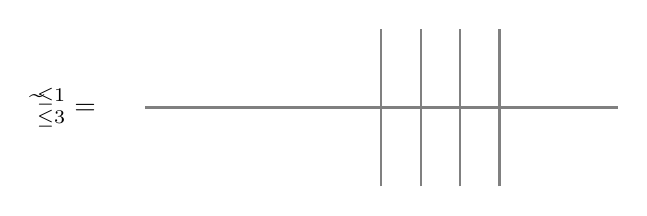
\begin{tikzpicture}
\draw[gray, thick] (-3,0) -- (3,0);
\draw[gray, thick] (0,-1) -- (0,1);
\draw[gray, thick] (.5,-1) -- (.5,1);
\draw[gray, thick] (1,-1) -- (1,1);
\draw[gray, thick] (1.5,-1) -- (1.5,1);
\node at (-4, 0)   (a) {$\widetilde{\sZ}_{\leq 3}^{\leq 1} = $} ;
\end{tikzpicture}
\]

\noindent where the horizontal axis is the $b_{-1}$-axis, and the fiber
over $b_{-1} = i$ is given the coordinate $a_i$.

The structural maps $\widetilde{\sZ}_{\leq m+1}^{\leq 1} \to 
\widetilde{\sZ}_{\leq m}^{\leq 1}$ coming from the 
embedding $A_{1,\leq m} \into A_{1,\leq m+1}$ correspond to contracting 
the rightmost line in the picture. Therefore, as:
%
\[
\widetilde{\sZ}^{\leq 1} = \underset{m}{\lim} \, \widetilde{\sZ}_{\leq m}^{\leq 1}
\]

\noindent we obtain the picture:
%
\[
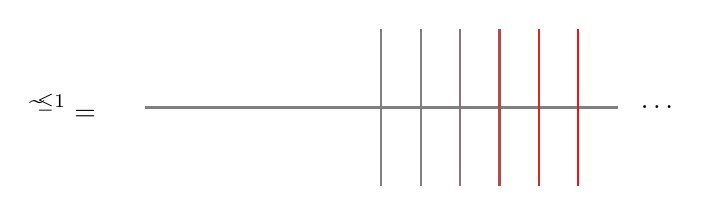
\begin{tikzpicture}
\draw[gray, thick] (-3,0) -- (3,0);
\draw[gray, thick] (0,-1) -- (0,1);
\draw[gray, thick] (.5,-1) -- (.5,1);
\draw[gray!90!red, thick] (1,-1) -- (1,1);
\draw[gray!60!red, thick] (1.5,-1) -- (1.5,1);
\draw[gray!30!red, thick] (2,-1) -- (2,1);
\draw[gray!15!red, thick] (2.5,-1) -- (2.5,1);
\node at (-4, 0)   (a) {$\widetilde{\sZ}^{\leq 1} = $} ;
\node at (3.5, 0)   (b) {$\ldots$} ;
\end{tikzpicture}
\]

\noindent where the reddening indicates that interpret the
picture in the \emph{pro}-sense rather than the \emph{ind}-sense.

\begin{rem}
\source{tates-thesis-de-rham-setting}
\notready

For $n > 1$, the stack $\sZ^{\leq n}$ is non-reduced, so there
is additional complexity in attempting to draw pictures.
(In addition, its Krull dimension grows with $n$.)

\end{rem}

\subsubsection{}

The map $\iota:\widetilde{\sZ}^{\leq 1} \to \widetilde{\sZ}^{\leq 1}$ 
corresponds to a rightward
shift in the above picture. Therefore,
if we let $\widetilde{\sY}_{\log}^{\leq 1}$ similarly be the total space
of the $\bG_m$-torsor over $\sY_{\log}^{\leq 1}$, 
from \eqref{eq:y-log-colim-iota} we obtain the picture:
%
\[
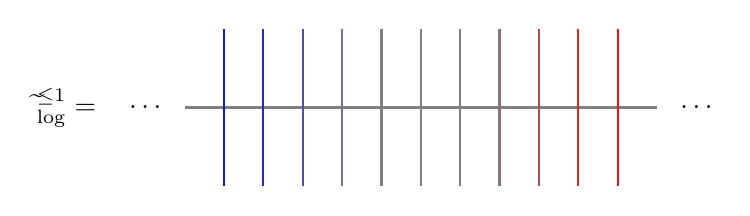
\begin{tikzpicture}
\draw[gray, thick] (-3,0) -- (3,0);
\draw[gray, thick] (0,-1) -- (0,1);
\draw[gray, thick] (.5,-1) -- (.5,1);
\draw[gray!90!red, thick] (1,-1) -- (1,1);
\draw[gray!60!red, thick] (1.5,-1) -- (1.5,1);
\draw[gray!30!red, thick] (2,-1) -- (2,1);
\draw[gray!15!red, thick] (2.5,-1) -- (2.5,1);
\draw[gray, thick] (-.5,-1) -- (-.5,1);
\draw[gray!90!blue, thick] (-1,-1) -- (-1,1);
\draw[gray!60!blue, thick] (-1.5,-1) -- (-1.5,1);
\draw[gray!30!blue, thick] (-2,-1) -- (-2,1);
\draw[gray!15!blue, thick] (-2.5,-1) -- (-2.5,1);
\node at (-4.5, 0)   (a) {$\widetilde{\sY}_{\log}^{\leq 1} = $} ;
\node at (3.5, 0)   (b) {$\ldots$} ;
\node at (-3.5, 0)   (b) {$\ldots$} ;
\end{tikzpicture}
\]

\noindent where the bluing in the picture indicates that we interpret
the limit in the \emph{ind}-sense (and the reddening is as before).

Informally, $\widetilde{\sY}_{\log}^{\leq 1}$ is a \emph{semi-infinite comb}. It has
infinitely many bristles, which are attached to the handle at integer
points; in the positive direction, these bristles have
pro-nature, and in the negative direction they have ind-nature.\footnote{We 
are unfortunately unable to produce non-synesthetic
pictures adequately distinguishing between projective and inductive limits. 
If asked to better explain the above pictures, 
we would resort to the formal descriptions
$\sZ^{\leq 1} = \lim_m \sZ_{\leq m}^{\leq 1}$ and $\sY_{\log}^{\leq 1} = 
\colim_{\iota} \sZ^{\leq 1}$.}

\subsubsection{}

In each of these pictures, $\bG_m$ acts by scaling in the vertical direction, i.e.,
scaling the bristles. So forming stacky quotients for this action, 
we obtain the promised sketches of 
$\sZ^{\leq 1}$ and $\sY_{\log}^{\leq 1}$.

Finally, the action of $\bZ = \Gr_{\bG_m}^{\leq 1}$ on $\sY_{\log}$ is generated
by rightward shift in the above pictures. Quotienting by this action gives a 
picture\footnote{Roughly speaking, this picture looks like $\bA^1/\bZ$ with a 
single bristle attached at $\bZ/\bZ$. But we must not forget the semi-infinite nature
of that bristle, which we find difficult to visually express in this setting.} 
for $\sY^{\leq 1}$.
